\section{Modellazione tramite Reti di Petri}
Per descrivere e validare formalmente la logica di sincronizzazione e controllo, sono state sviluppate due Reti di Petri focalizzate sugli aspetti critici del sistema.

\subsection{ActiveController e Polling asincrono}
\begin{figure}[H]
    \centering
    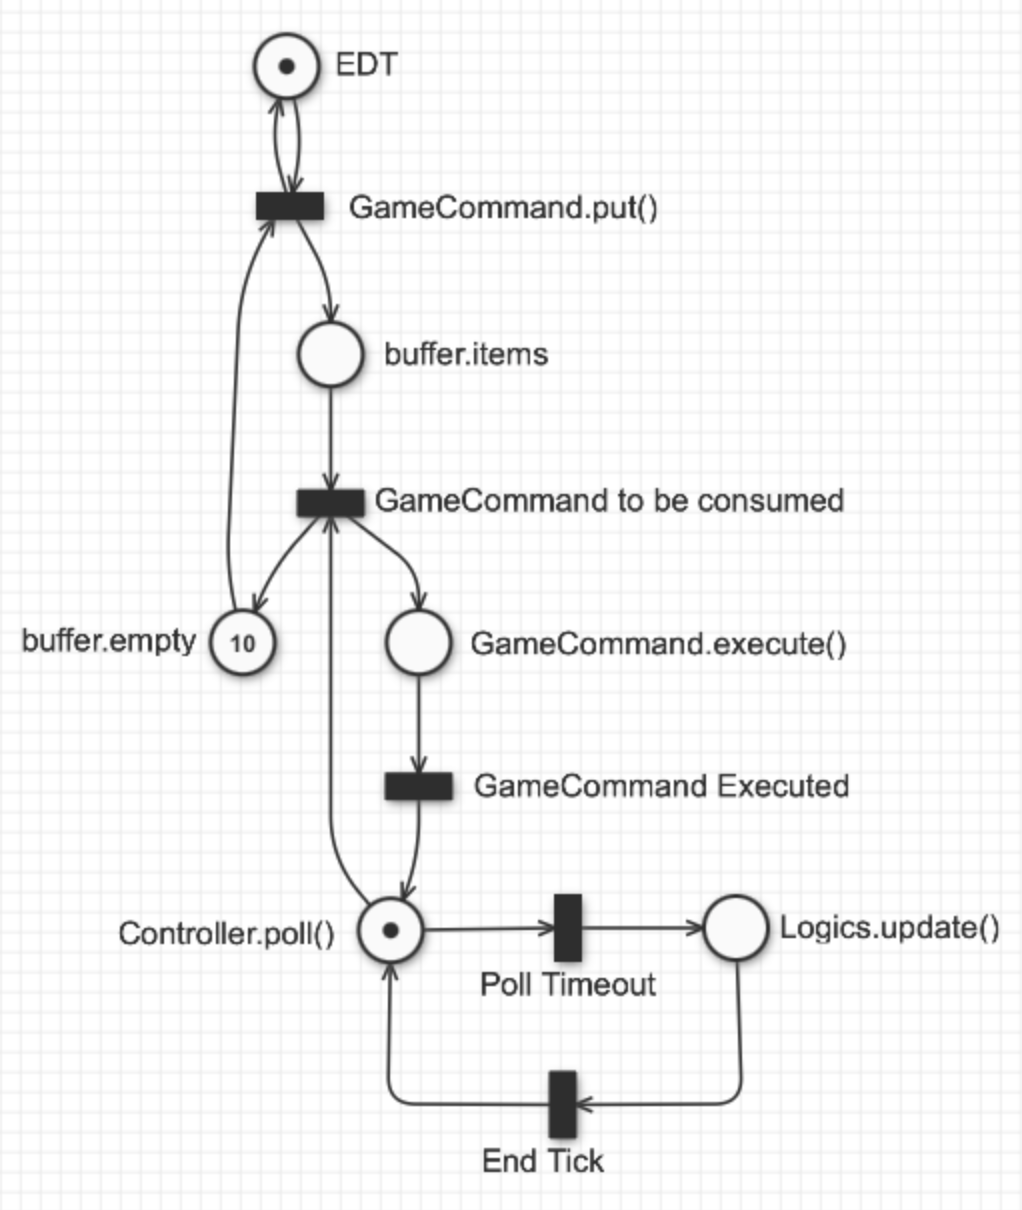
\includegraphics[width=0.7\linewidth]{figures/activeController.png}
    \caption{Rete di Petri: interazione tra EDT e ActiveController tramite BoundedBuffer.}
    \label{fig:pn_active_controller}
\end{figure}

La rete in Figura \ref{fig:pn_active_controller} astrae il coordinamento tra la UI e il \texttt{GameLoop}. L'analisi formale verifica le proprietà di \textbf{k-Boundedness}, poichè il numero di token in \texttt{buffer.items} è limitato dalla capacità assegnata (in \texttt{buffer.empty}).
La \textbf{Liveness} della rete dimostra la totale assenza di deadlock. La transizione autonoma di \texttt{Poll(waitMs)} evita attese infinite in caso di buffer vuoto, garantendo che i \emph{tick} fisici vengano ciclicamente eseguiti.

\subsection{Collisioni Multithreading}
\begin{figure}[H]
    \centering
    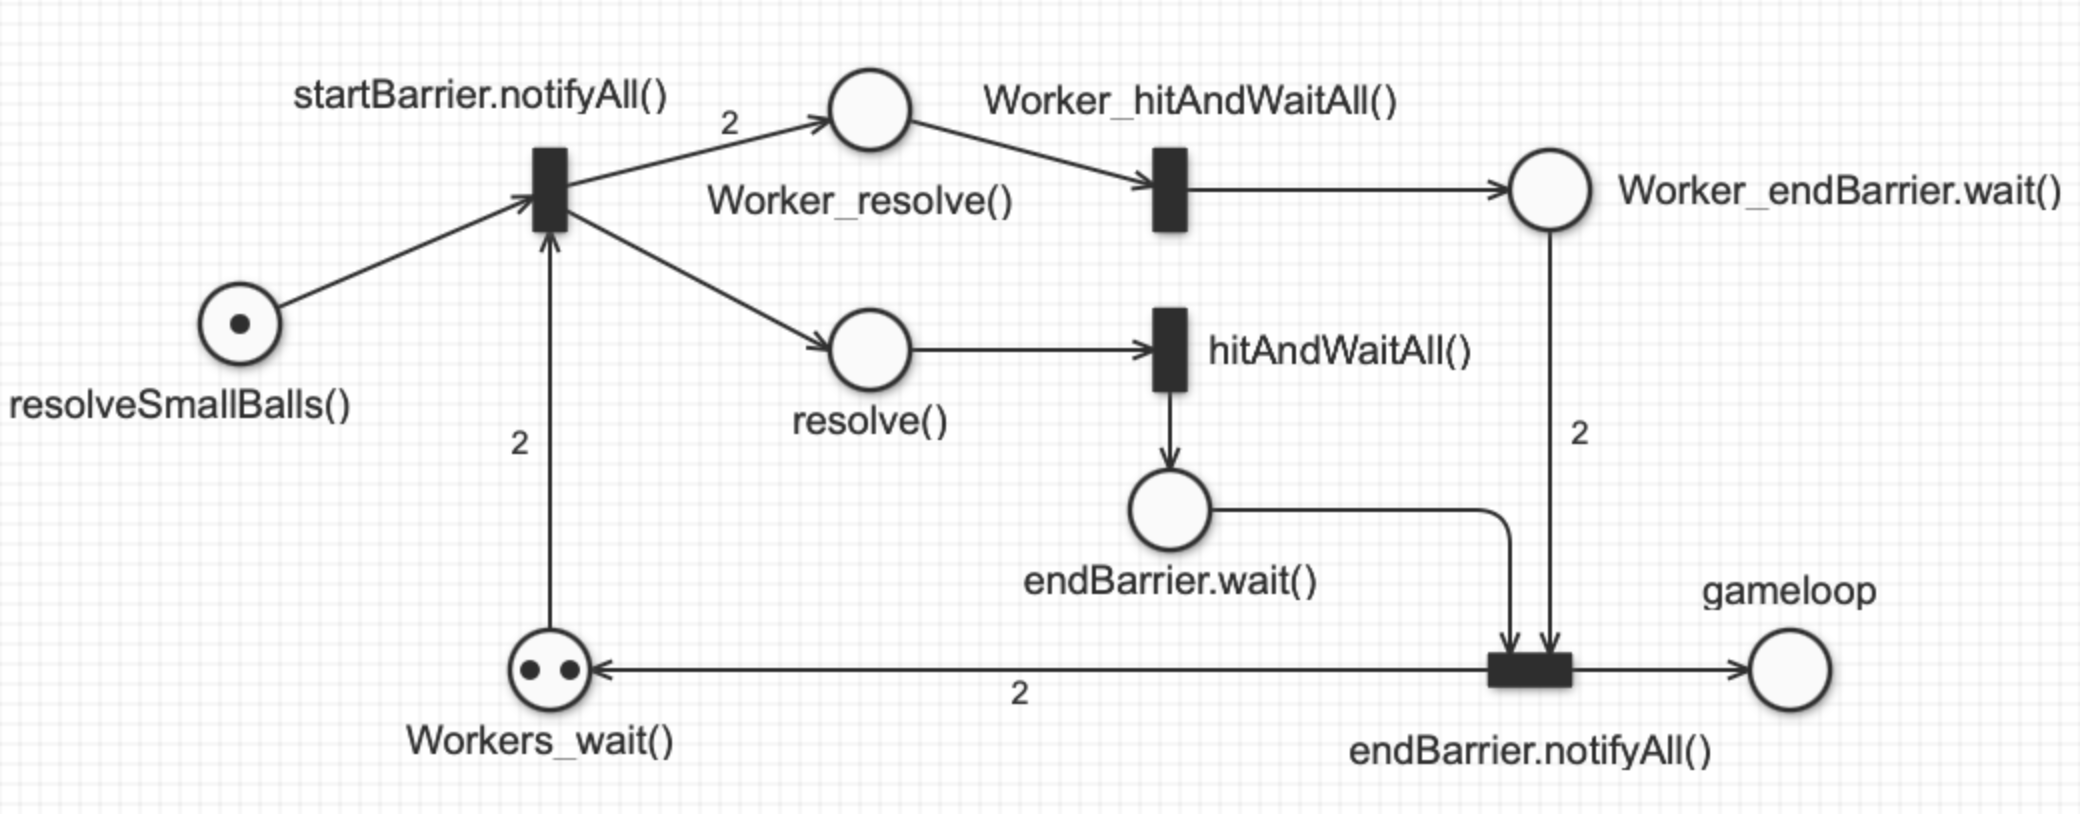
\includegraphics[width=0.8\linewidth]{figures/collisions.png}
    \caption{Rete di Petri: Risoluzioni delle collisioni con CyclicBarrier.}
    \label{fig:pn_collisions}
\end{figure}

La Figura \ref{fig:pn_collisions} astrae il meccanismo di risoluzione delle collisioni utilizzando un \textbf{CyclicBarrier}.
La rete evidenzia la sincronizzazione tra il thread Master e i Worker durante la fase di calcolo delle collisioni. La proprietà di \textbf{Liveness} è garantita dalla struttura ciclica della rete ogni Worker e il Master, una volta completato il proprio lavoro, attende sulla barriera; La rete mostra come è necessario che tutti i token (pari numero dei worker e del Master) raggiungano la barriera prima che essa notifica il risveglio, e l'\texttt{ActiveController} possa procedere con un successivo \textbf{Gameloop}, assicurando così la coerenza dello stato del gioco prima di ogni rendering.
Il numero di token e i pesi delle transizioni sono impostati a $2$ ma possono essere scalati per rappresentare un numero arbitrario di Worker, mantenendo invariata la logica di sincronizzazione e garantendo sempre le stesse proprietà formali.

\newpage
\subsection{Prevenzione Deadlock tramite Lock Ordering}
\begin{figure}[H]
    \centering
    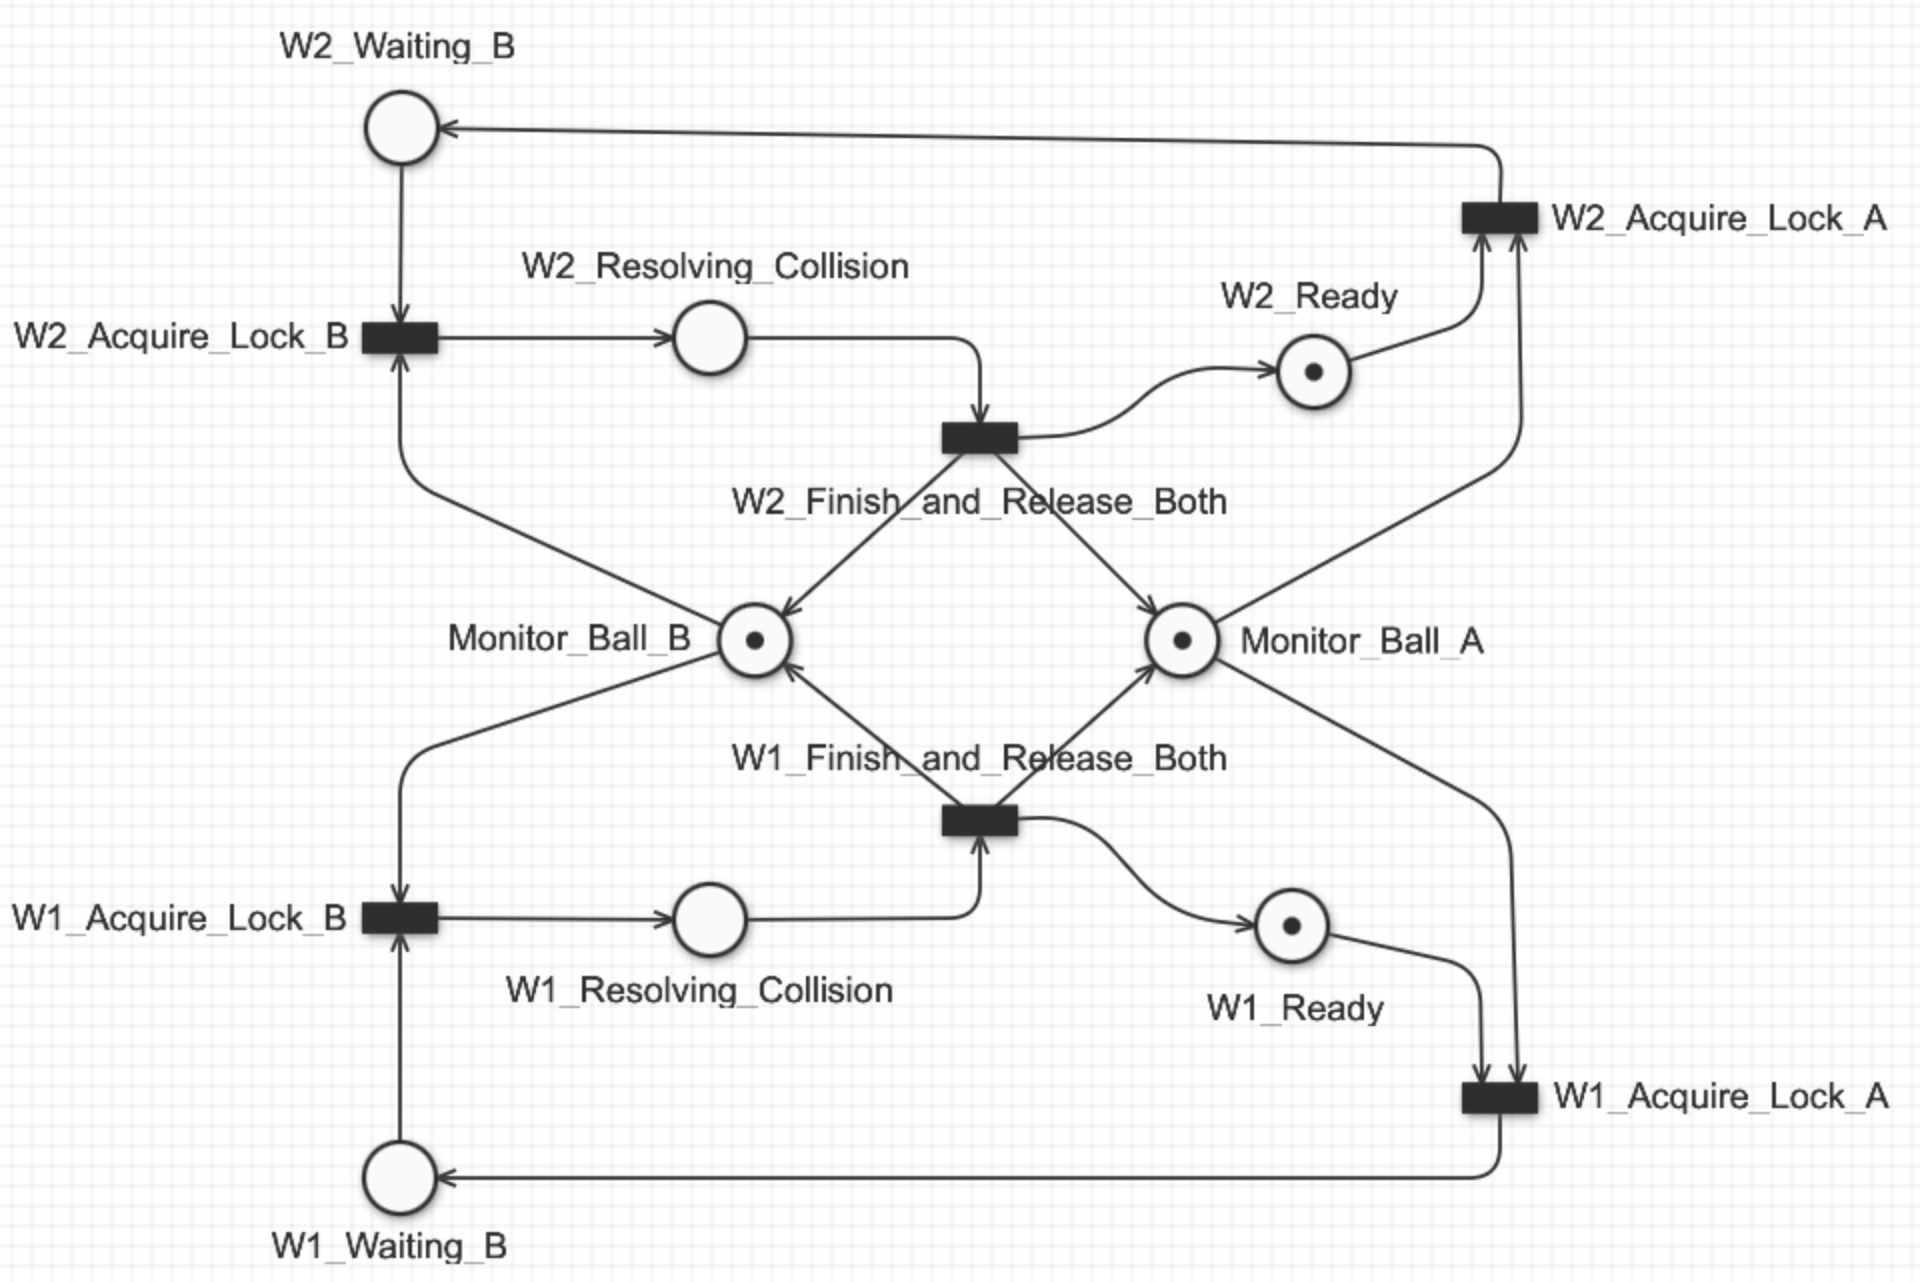
\includegraphics[width=0.8\linewidth]{figures/lock_ordering.png}
    \caption{Rete di Petri: Lock Ordering durante la verifica concorrente delle collisioni.}
    \label{fig:pn_lock_ordering}
\end{figure}

La Figura \ref{fig:pn_lock_ordering} astrae due worker concorrenti in competizione per le due Ball (\texttt{Monitor\_Ball\_A} e \texttt{Monitor\_Ball\_B}). 
L'introduzione di un ordine deterministico impone che l'acquisizione del primo lock diventi uno step obbligato e mutuamente esclusivo. Il worker sconfitto nella contesa per il primo lock resta in \emph{Ready}, permettendo al thread vincente di procedere indisturbato verso l'acquisizione dell'ultimo lock.
La rete è priva di \textbf{Deadlock} poichè non esistono configurazioni raggiungibili della rete in cui subentri l'attesa circolare. L'esecuzione si dimostra ciclica e robusta a prescindere dal livello di asincronia tra i task.